% Part: sets-functions-relations
% Chapter: arithmetization
% Section:reals

\documentclass[../../../include/open-logic-section]{subfiles}

\begin{document}

\olfileid[tr]{sfr}{arith}{real}
\olsection{Gerçel Sayı Doğrusu}

Sonraki adım, gerçel sayıların rasyonel sayılardan nasıl kurulacağını göstermektir.
Bundan önce gerçel sayıların \emph{ayırt edici} özelliğini anlamamız gerekir.

Gerçel sayılar rasyonel sayılara çok benzer biçimde davranır. (Teknik olarak
ikisi de \emph{sıralı cisim} örneğidir; bunun tanımı için
\olref[check]{orderedfield}'e bakın.) Şimdi, \olref[sfr][siz][]{chap}'ın
alıştırmalarını yaptıysanız gerçel sayıların rasyonel sayılardan kesinlikle daha
çok olduğunu, yani $\cardless{\Rat}{\Real}$ olduğunu biliyorsunuzdur. Bunu ilk
kez Cantor ispatladı. Ancak irrasyonel sayıların, yani rasyonel olmayan gerçel
sayıların varlığı yaklaşık iki buçuk bin yıldır bilinmektedir. Nitekim:
%\footnote{Now: “$\sqrt{2}$” equally refers to both the positive and the negative roots; but in the next few pages, I'll forget about this, and consider only the positive root.}
\begin{thm}\ollabel{root2irrational}
$\sqrt{2}$ rasyonel değildir; yani $\sqrt{2} \notin \Rat$.
\end{thm}

\begin{proof}
Olmayana ergiyle, $\sqrt{2}$'nin rasyonel olduğunu varsayalım. Öyleyse bazı
pozitif $m$ ve $n$ doğal sayıları için $\sqrt{2} = \nicefrac{m}{n}$ olur.
Üstelik $m$ ve $n$'yi kesir daha fazla sadeleştirilemeyecek biçimde
seçebiliriz.
Düzenlersek $m^{2} = 2n^{2}$ elde edilir. Buradan ispatı iki yolla
tamamlayabiliriz:

\emph{Birincisi, geometrik olarak} (Tennenbaum'u izleyerek).\footnote{Bu ispatı
\cite{Conway2006} aktarır.} Şu kareleri ele alın:
\begin{center}	
	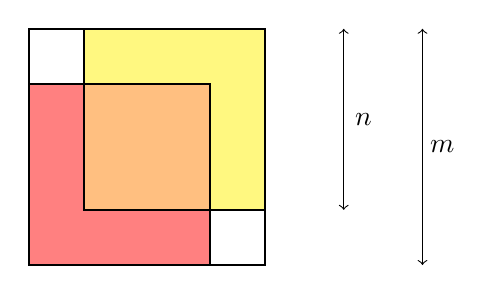
\begin{tikzpicture}
		\draw[thick] (0,0) rectangle (3,3);
		\draw[thick, fill=red!50] (0,0) rectangle (2.3,2.3);
		\draw[thick, fill=yellow!50] (0.7,0.7) rectangle (3, 3);
		\draw[thick, fill=orange!50] (0.7,0.7) rectangle (2.3, 2.3);
		\draw[<->] (4, 0.7)--(4, 3);
		\node at (4.25, 1.85) (n) {$n$};
		\draw[<->] (5, 0)--(5, 3);
		\node at (5.25, 1.5) (m) {$m$};
	\end{tikzpicture}
\end{center}
$m^2 = 2n^2$ olduğundan, kenarı $n$ olan iki karenin örtüştüğü bölgenin
alanı, iki karenin de kaplamadığı bölgenin alanına eşittir; yani turuncu
karenin alanı, gölgesiz iki karenin alanları toplamına eşittir. Turuncu
karenin kenarı $p$, gölgesiz karelerin her birinin kenarı $q$ ise
$p^2 = 2q^2$ olur. Fakat şimdi $p < m$, $q < n$ ve $p, q \in \Nat$ olmak
üzere $\sqrt{2} = \nicefrac{p}{q}$'dur. Bu, $m$ ve $n$'nin başlangıçtaki
kesir daha fazla sadeleştirilemeyecek biçimde seçilmiş olmasıyla çelişir.
		
\emph{İkincisi, biçimsel olarak.} $m^{2} = 2n^{2}$ olduğundan $m$ çifttir.
($x$ tekse $x^2$'nin de tek olduğunu göstermek kolaydır.) Öyleyse bazı
$r \in \Nat$ için $m = 2r$ olur. Yeniden düzenleyince $2r^2 = n^2$ elde
edilir,
		%				\begin{align*}
		%					(2q)^{2} &= 2n^{2}\\
		%					4q^{2} &= 2n^{2}\\
		%					2q^{2} &= n^{2}
		%				\end{align*}
dolayısıyla $n$ de çifttir. Böylece hem $m$ hem $n$ çifttir ve
$\nicefrac{m}{n}$ kesri \emph{daha fazla} sadeleştirilebilir. Çelişki!
\end{proof}

Yeri gelmişken bu diyagramsal ispat, tarih bölümündeki “Tarihten Çok Mit mi?”
başlıklı kısımda ele alınan malzemeye yeniden dönmemizi sağlar. Tennenbaum
(1927--2006) bütünüyle modern
bir matematikçiydi; yine de ispat inkâr edilemeyecek kadar güzel, tümüyle
titiz ve geometrik sezgiye başvuruyor!

Her hâlükârda gerçel sayılar rasyonel sayılardan “daha kapsamlıdır”. Bir
anlamda rasyonel sayılarda “boşluklar” vardır ve gerçel sayılar bu boşlukları
doldurur. Weierstrass bunun, gerçel sayıları rasyonel sayılardan ayıran tek bir
özelliği, yani Tamlık Özelliği'ni betimlediğini fark etti:
\emph{Üstten sınırlı ve boş olmayan her gerçel sayı kümesinin en küçük bir üst
sınırı vardır.}

Rasyonel sayıların Tamlık Özelliği'ne sahip olmadığını görmek kolaydır.
Örneğin $\sqrt{2}$'den küçük rasyonel sayılar kümesini ele alın:
\[
	\Setabs{p \in \Rat}{p^2 < 2 \text{ veya }p < 0}
\]
Bu kümenin rasyonel sayılar içinde bir üst sınırı vardır; örneğin
!!{element}larının hepsi $3$'ten küçüktür. Peki en küçük üst sınırı nedir?
$\sqrt{2}$ demek isteriz; fakat az önce $\sqrt{2}$'nin \emph{rasyonel
olmadığını} gördük. Ayrıca $\sqrt{2}$'den büyük \emph{en küçük} bir rasyonel
sayı yoktur. Demek ki kümenin bir üst sınırı vardır ama en küçük üst sınırı
yoktur. Dolayısıyla rasyonel sayılar Tamlık Özelliği'nden yoksundur.

Buna karşılık kontinuumun Tamlık Özelliği'ne “özü gereği sahip olması”
beklenir. Yalnızca $\sqrt{2}$'nin bir gerçel sayı olmasını istemeyiz; rasyonel
sayı doğrusundaki bütün “boşlukları” doldurmak isteriz. Dahası, kontinuumun
kendisinde hiçbir “boşluk” bulunmamasını isteriz. Tamlık aracılığıyla elde
edeceğimiz tam da budur.

\end{document}
